% !TEX root = morphkasten.tex

\section{Lenkung}


%############## Trapez
\subsection{Trapez}

\begin{figure} [hbp]
	\centering
	\begin{subfigure}[b]{0.4\textwidth}
		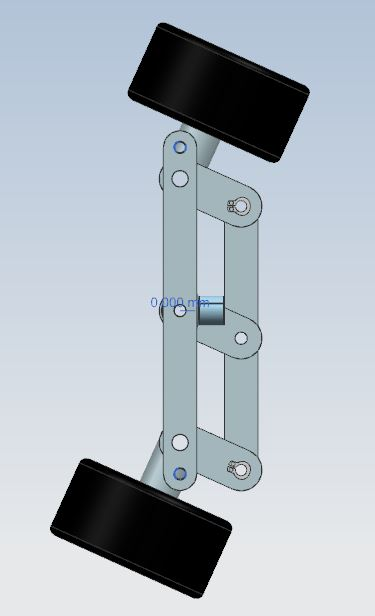
\includegraphics[width=0.8\textwidth]{fig/Trapezlenkung3.JPG}
		\caption{1. Situation: CAD-Modell}
	\end{subfigure}
	\hfill
	\begin{subfigure}[b]{0.36\textwidth}
		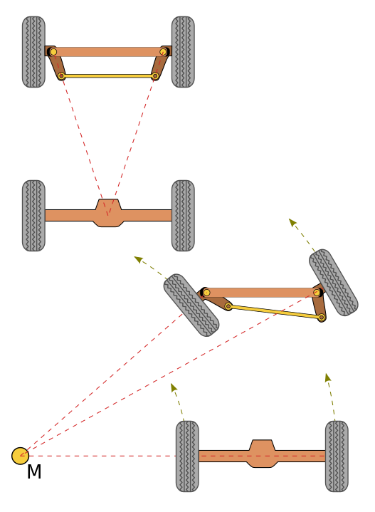
\includegraphics[width=\textwidth]{fig/Lenktrapez.png}
		\caption{2. Situation: Trapezlenkung
		(Quelle: http://www.portmanns.ch/Repetition/ \\
		Fahrwerk/Lenkungsarten.pdf)}
\end{subfigure}
	\caption{Trapezlenkung}\label{fig:animals}
\end{figure}

\begin{table}[h]
\begin{tabular}{p{0.5\textwidth} | p{0.5\textwidth}}


 \textbf{Vorteile} & \textbf{Nachteile} \\ \hline
	 
\begin{itemize}
\item Konventionelle, oft verwendete Lenkung für PWS
\item Berechnungen für Lenkgeometrie im Internet
\item Viele reale Beispiele als Vorlage
\end{itemize}

 
 &
 
\begin{itemize}
\item Herstellung relativ aufwändig
\item Kamera ist in der Kurve nicht gerade zur Strecke
\end{itemize}

\end{tabular}
\end{table}

\begin{table}[h]
\begin{tabular}{p{0.5\textwidth}p{0.5\textwidth}}


 \textbf{Risiken} & \\ \hline
	 
\begin{itemize}
\item Die Lenkung könnte zu unpräzise sein um einen genauen Abstand zum Trottoir zu halten.
\end{itemize}


 
\end{tabular}
\end{table}

\pagebreak


%############## Raupen
\subsection{Raupen}
Im Kapitel 1.1 wurden die Variante Raupen bereits beschrieben.


%############## 2 Räder mit 2 Motoren
\subsection{2 Räder mit 2 Motoren}

\begin{figure}[h!]%Position festigen
\centering
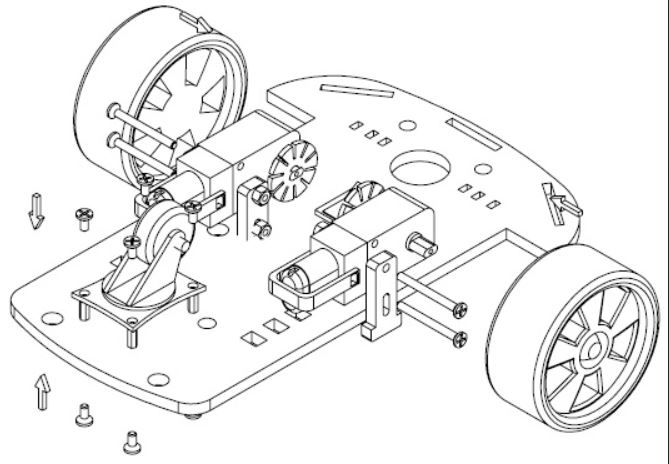
\includegraphics[width=0.6\textwidth]{fig/3rad-3.JPG}
\caption{2-Rad mit Stützen (Quelle:www.sainsmart.com)}
\label{fig:2-Rad mit Stützen}
\end{figure}


\begin{table}[h]
\begin{tabular}{p{0.5\textwidth} | p{0.5\textwidth}}


 \textbf{Vorteile} & \textbf{Nachteile} \\ \hline
	 
\begin{itemize}
\item Wendig
\item Kamera gerade zur Strecke
\item Vorwissen für die Regelung durch MC-Modul an der HSLU
\item Konstruktiv einfach realisierbar
\end{itemize}

 
 &
 
\begin{itemize}
\item Geringe Stabilität
\item Motoren müssen sehr genau sein
\item Aufwändige Regelung
\end{itemize}

\end{tabular}
\end{table}

\begin{table}[h]
\begin{tabular}{p{0.5\textwidth}p{0.5\textwidth}}


 \textbf{Risiken} & \\ \hline
	 
\begin{itemize}
\item Bei einem 2-Rad Modell ist die Stabilität ein Problem. Beim Aufladen des Containers könnte das Fahrzeug kippen.
\end{itemize}
&
\begin{itemize}
\item Wenn die Antriebsräder in der Mitte montiert sind, braucht man vorne und hinten ein Stützrad oder eine Stützkugel. Diese könnten grössere Reibungskräfte verursachen.
\end{itemize}


 
\end{tabular}
\end{table}

\pagebreak